In this section, we illustrate the performance of the Saltelli SI estimators using stochastic QoIs with and without a variance deconvolution correction. 
We first discuss results for a test case with an analytic solution and then test the method on a radiation transport example problem.

\subsection{Ishigami function}
To test the accuracy of the derived estimators against analytic solutions, we add a stochastic parameter to the test function from Ishigami and Homma~\cite{ishigami-homma-1990}:
\begin{gather} \label{m2eq:stoch-ishigami}
    f \left( \xi_1, \xi_2, \xi_3, \eta \right) = \sin \left( \xi_1 \right) + a \sin^2 \left( \xi_2 \right) + b \xi_3^4 \sin \left( \xi_1 \right) + c\eta, \\
    a=1, b=0.1, c=5, \nonumber \\
    \eta \sim \mathcal{N} \left(0,1\right), \quad (\xi_1, \xi_2, \xi_3) \sim \mathcal{U} \left( -\pi,+\pi\right) , \nonumber
\end{gather}
where $\xi_1$, $\xi_2$, and $\xi_3$ are independent input parameters and $\eta$ represents some intrinsic randomness. 
Because we have defined $\eta$ with mean zero and variance 1, the expected value of $f$ is the expected value of the standard Ishigami function and the variance of $f$ is the variance of the standard Ishigami function plus a constant $c^2$. 
In Figures~\ref{fig:ishigami-s1}-\ref{fig:ishigami-t3}, we compare the accuracy of the variance deconvolution (Var-D) vs the standard approach (Brute-F) over 200 repetitions for all first- and total-order indices. 
We use a consistent number of samples $\Nxi = 10^3$ to study the effect of increasing the number of histories per sample $\Neta$.
In general, we see that the Var-D estimator is more accurate than the Brute-F estimator, but has a larger variance especially at lower $\Neta$. 
In some cases this leads to the Brute-F estimator out-performing the Var-D estimator, in particular when the first-order index is near zero as with $\S{2}$ and $\S{3}$.
With $\S{1}$, we can clearly see that the Brute-F approach under-estimates the first-order index. With $\T{2}$ and $\T{3}$, we see that the Brute-F over-estimates the total-order index.
\begin{figure}[b]
    \centering
    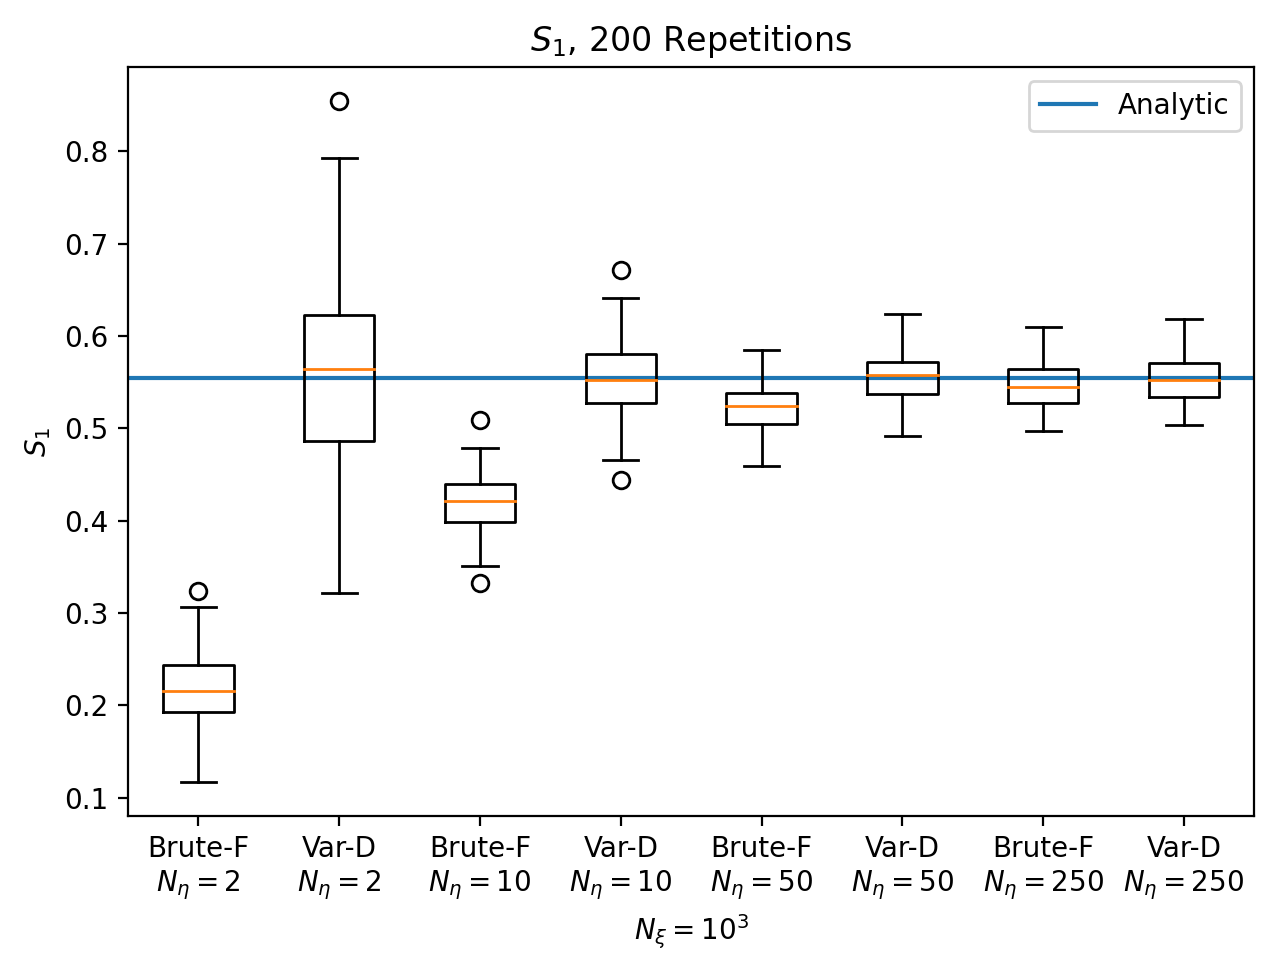
\includegraphics[width=\textwidth]{figures/ishi_s1_boxplot_c5.png}
    \caption{For the Ishigami function with added stochasticity, comparing distributions of $\S{1}$ calculated using a variance deconvolution (Var-D) vs. a standard approach (Brute-F) with the Saltelli estimator. $\Nxi=10^3$ in every case, with $\Neta$ increasing from left to right within a single plot. Analytic indices reported as solid horizontal line.}
    \label{fig:ishigami-s1}
\end{figure} \hfill
\begin{figure}[b]
    \centering
    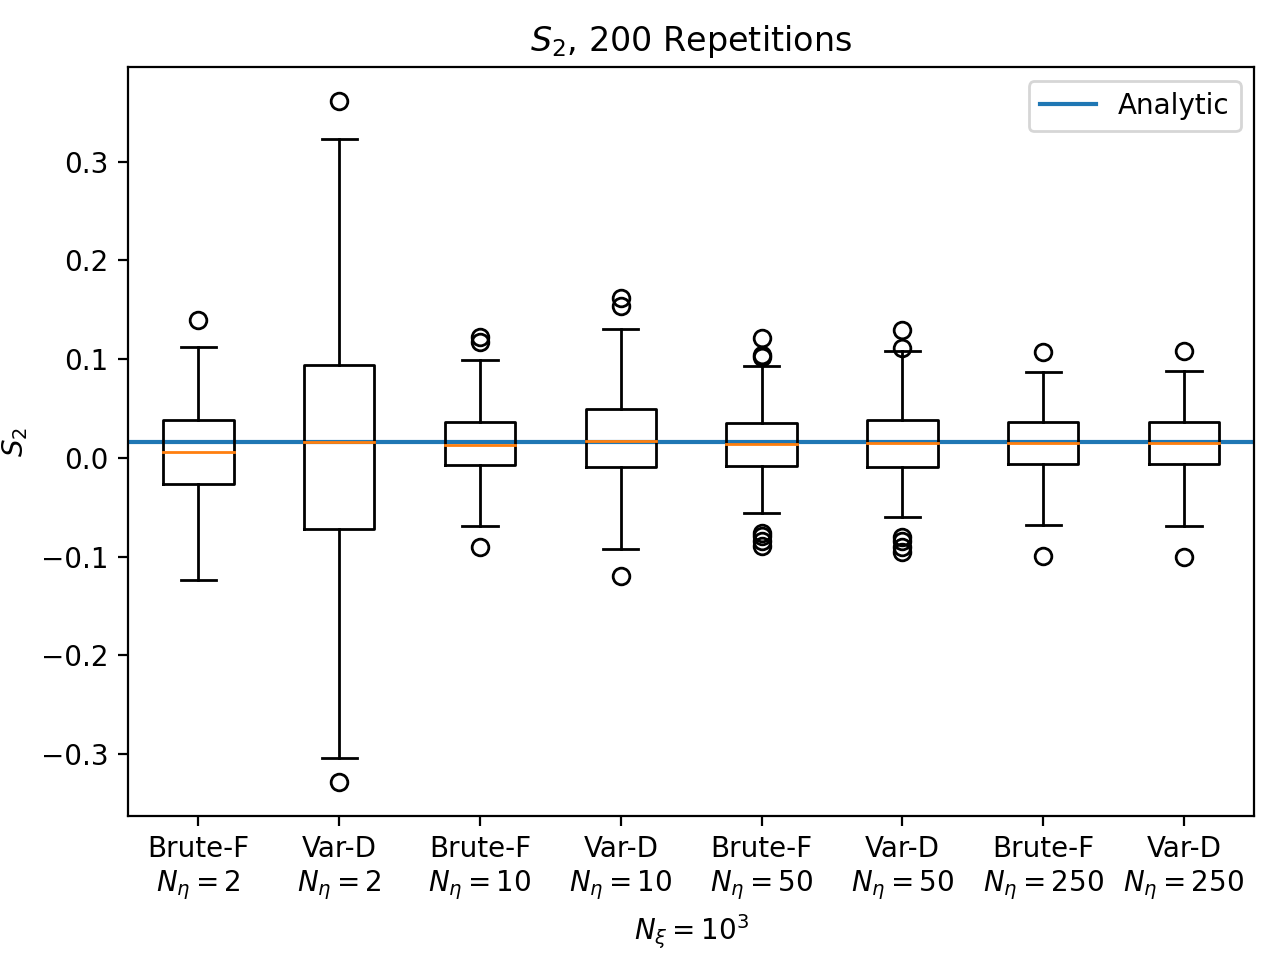
\includegraphics[width=\textwidth]{figures/ishi_s2_boxplot_c5.png}
    \caption{For the Ishigami function with added stochasticity, comparing distributions of $\S{2}$ calculated using a variance deconvolution (Var-D) vs. a standard approach (Brute-F) with the Saltelli estimator. $\Nxi=10^3$ in every case, with $\Neta$ increasing from left to right within a single plot. Analytic indices reported as solid horizontal line.}
    \label{fig:ishigami-s2}
\end{figure}
\begin{figure}[b]
    \centering
    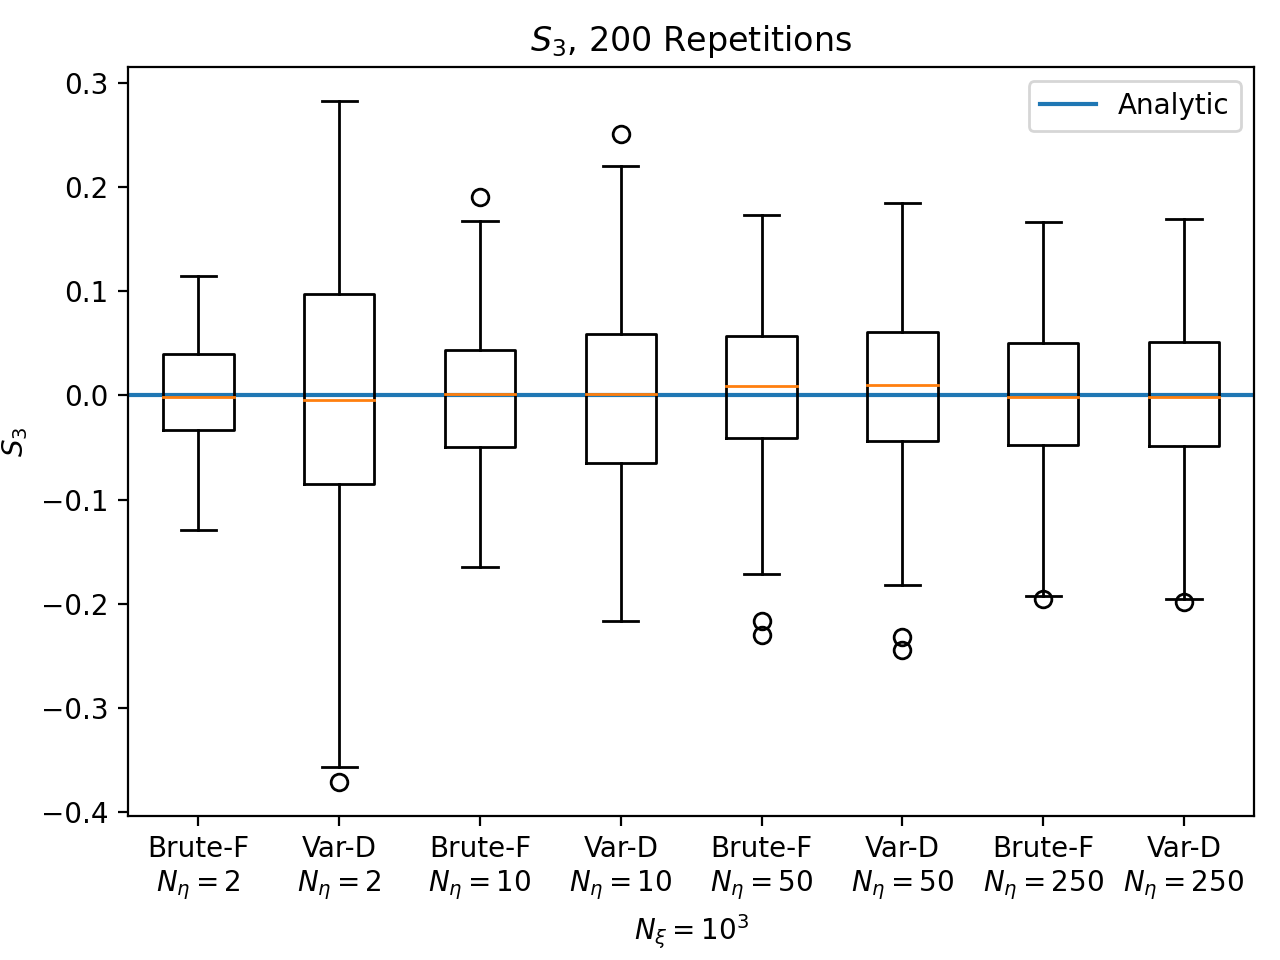
\includegraphics[width=\textwidth]{figures/ishi_s3_boxplot_c5.png}
    \caption{For the Ishigami function with added stochasticity, comparing distributions of $\S{3}$ calculated using a variance deconvolution (Var-D) vs. a standard approach (Brute-F) with the Saltelli estimator. $\Nxi=10^3$ in every case, with $\Neta$ increasing from left to right within a single plot. Analytic indices reported as solid horizontal line.}
    \label{fig:ishigami-s3}
\end{figure}
\begin{figure}[b]
    \centering
    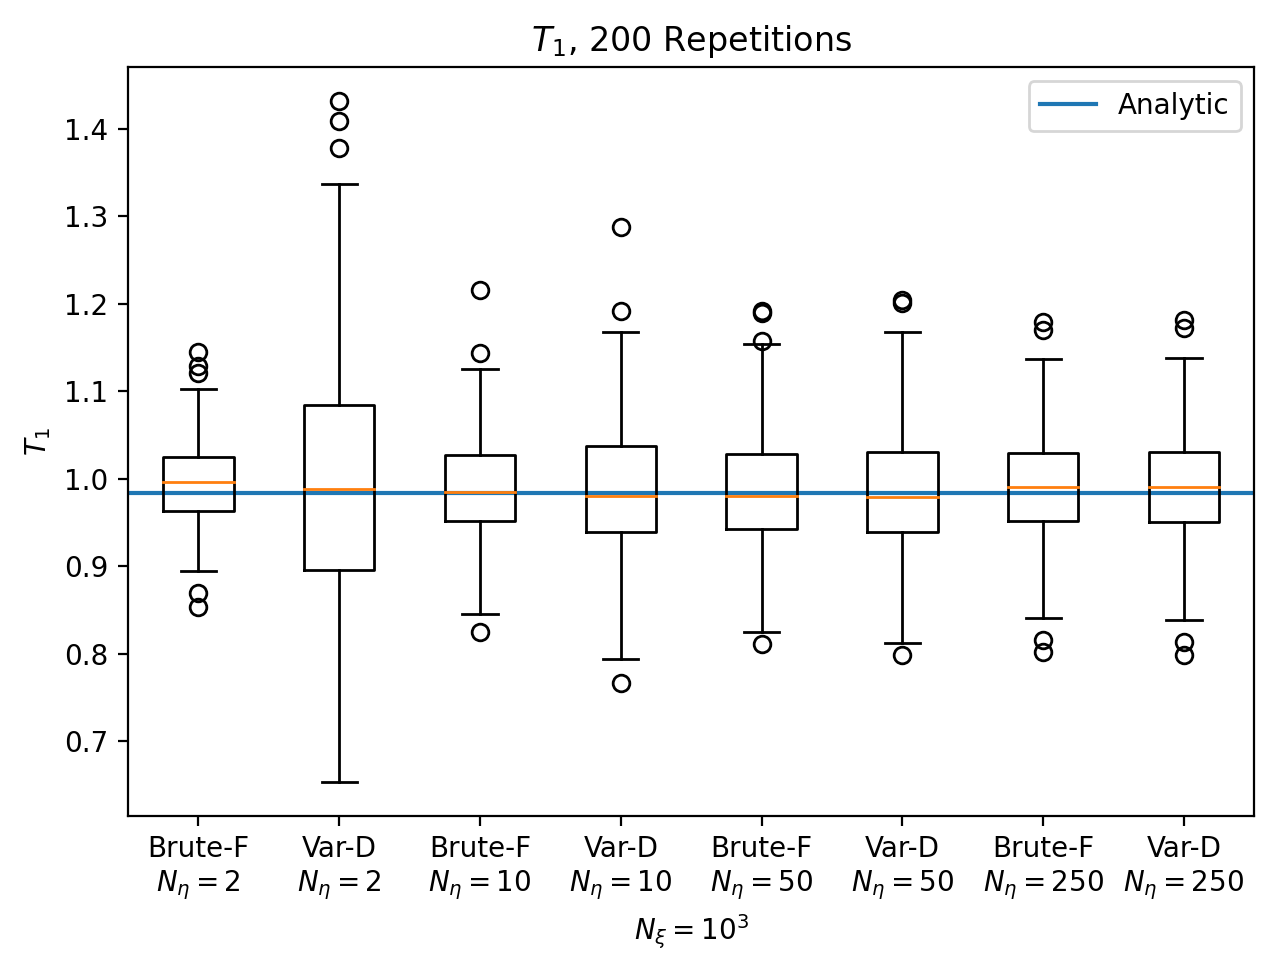
\includegraphics[width=\textwidth]{figures/ishi_t1_boxplot_c5.png}
    \caption{For the Ishigami function with added stochasticity, comparing distributions of $\T{1}$ calculated using a variance deconvolution (Var-D) vs. a standard approach (Brute-F) with the Saltelli estimator. $\Nxi=10^3$ in every case, with $\Neta$ increasing from left to right within a single plot. Analytic indices reported as solid horizontal line.}
    \label{fig:ishigami-t1}
\end{figure}
\begin{figure}[b]
    \centering
    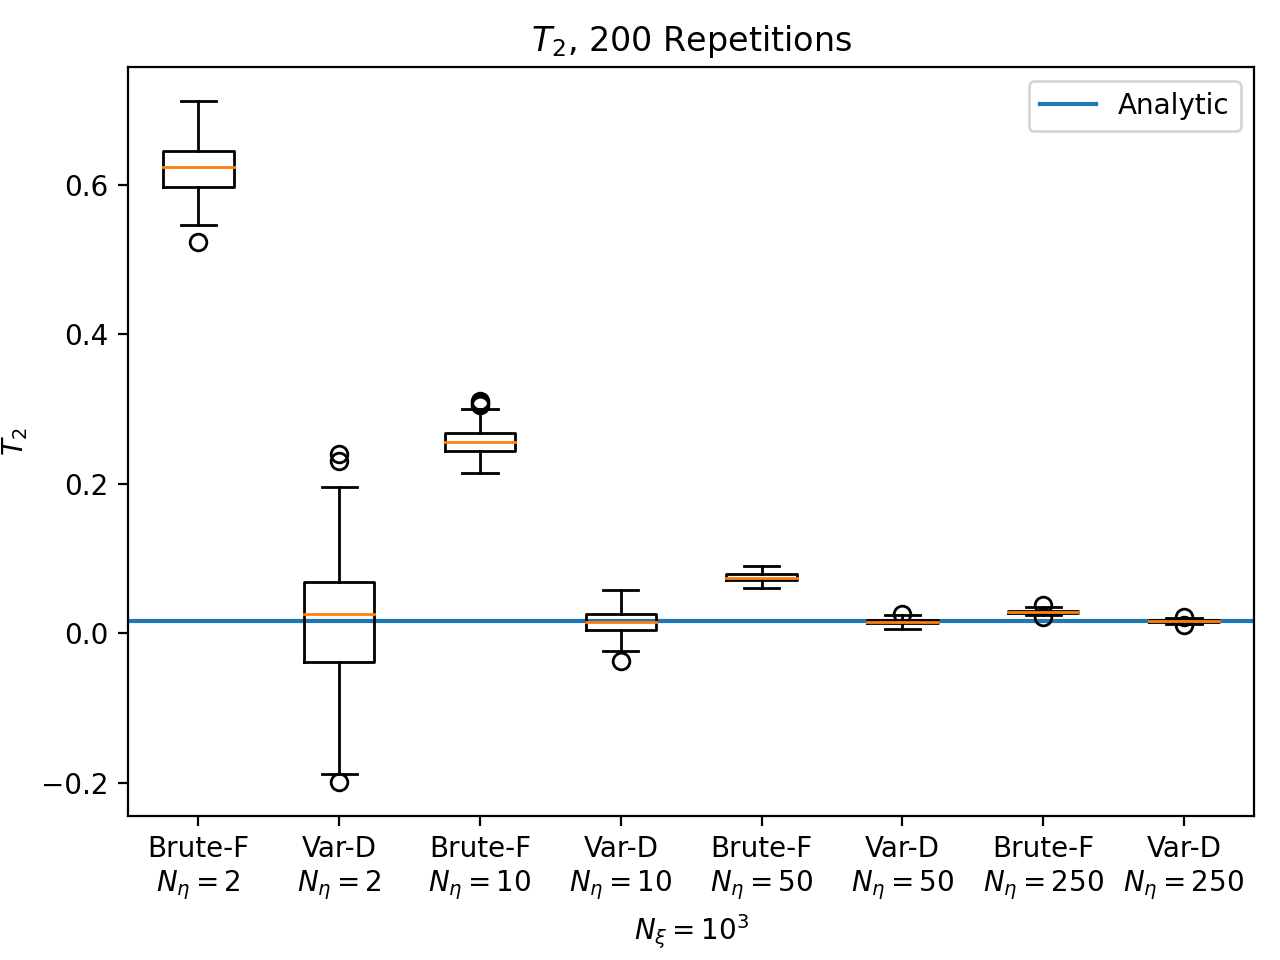
\includegraphics[width=\textwidth]{figures/ishi_t2_boxplot_c5.png}
    \caption{For the Ishigami function with added stochasticity, comparing distributions of $\T{2}$ calculated using a variance deconvolution (Var-D) vs. a standard approach (Brute-F) with the Saltelli estimator. $\Nxi=10^3$ in every case, with $\Neta$ increasing from left to right within a single plot. Analytic indices reported as solid horizontal line.}
    \label{fig:ishigami-t2}
\end{figure}
\begin{figure}[b]
    \centering
    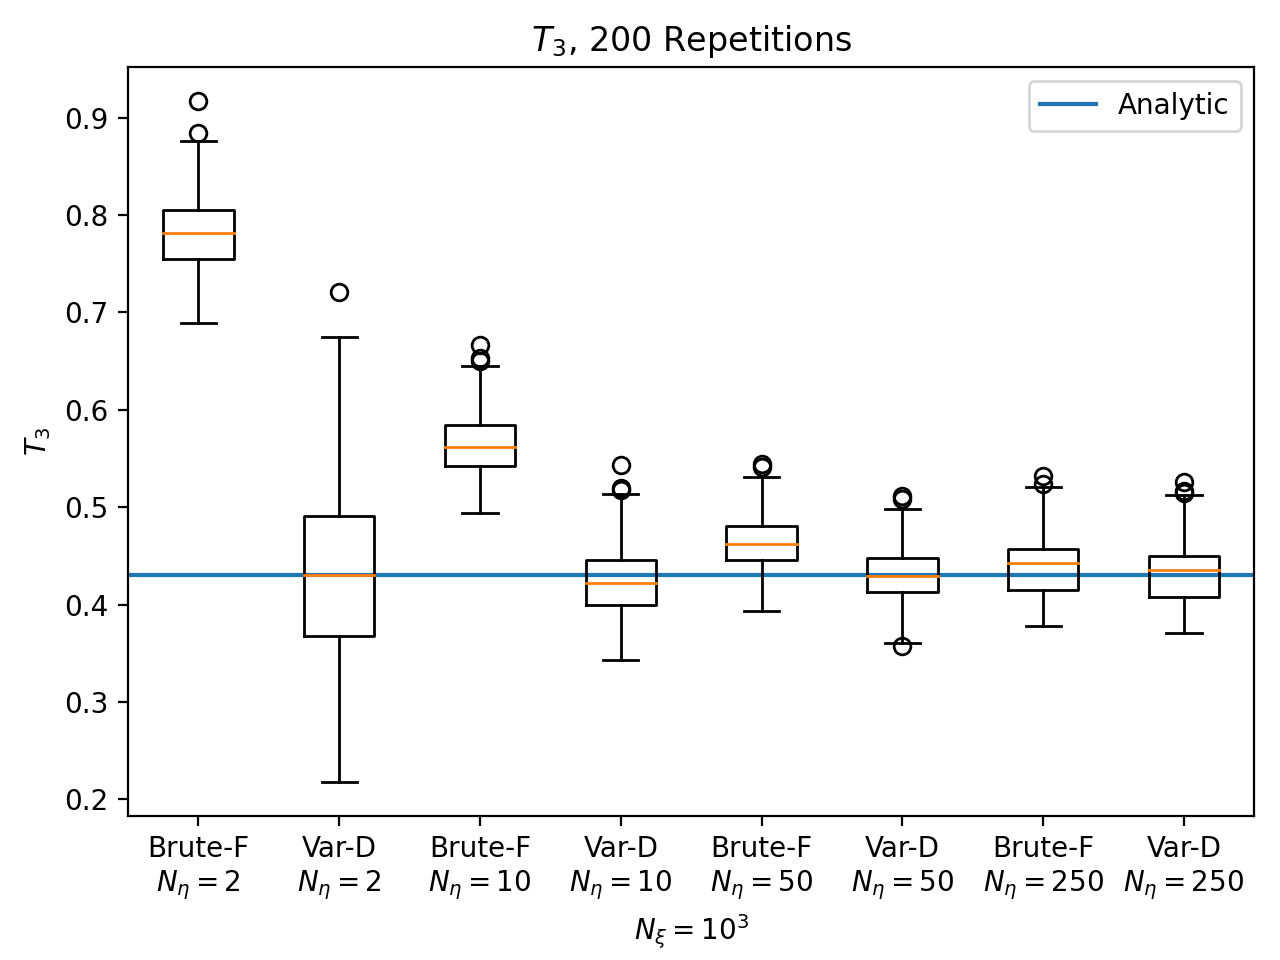
\includegraphics[width=\textwidth]{figures/ishi_t3_boxplot_c5.png}
    \caption{For the Ishigami function with added stochasticity, comparing distributions of $\T{3}$ calculated using a variance deconvolution (Var-D) vs. a standard approach (Brute-F) with the Saltelli estimator. $\Nxi=10^3$ in every case, with $\Neta$ increasing from left to right within a single plot. Analytic indices reported as solid horizontal line.}
    \label{fig:ishigami-t3}
\end{figure}

% \begin{figure}
% 	\centering
%     \begin{subfigure}[b]{0.3\textwidth}
%         \centering
%         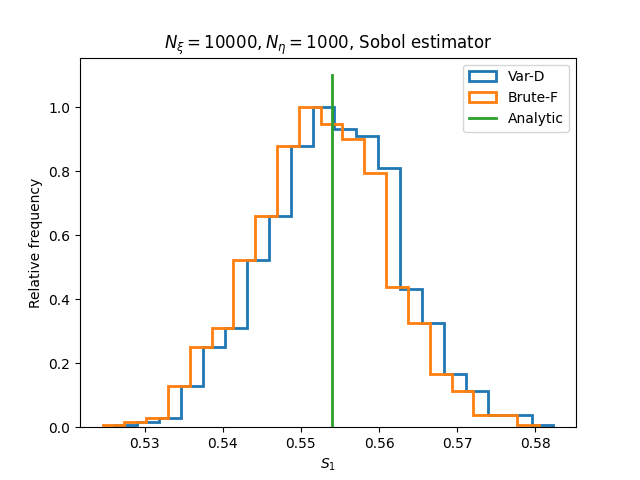
\includegraphics[width=\textwidth]{figures/s1_exp.png}
%         \caption{Computing $\S{1}$ using the Saltelli estimator.}
%         \label{fig:s1}
%     \end{subfigure} \hfill
%     \begin{subfigure}[b]{0.3\textwidth}
%         \centering
%         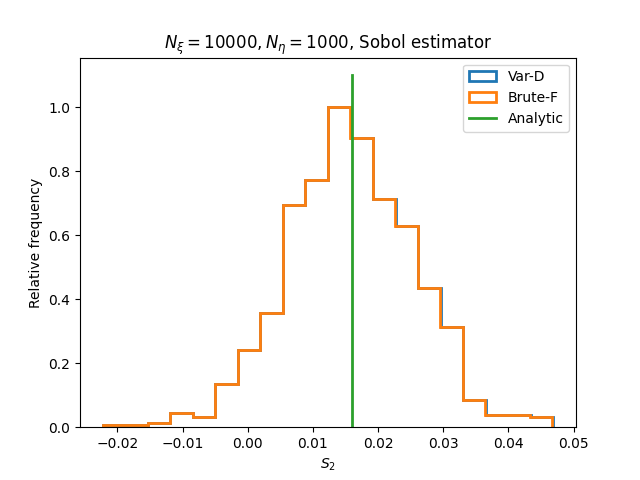
\includegraphics[width=\textwidth]{figures/s2_exp.png}
%         \caption{Computing $\S{2}$ using the Saltelli estimator.}
%         \label{fig:s1}
%     \end{subfigure} \hfill
%     \begin{subfigure}[b]{0.3\textwidth}
%         \centering
%         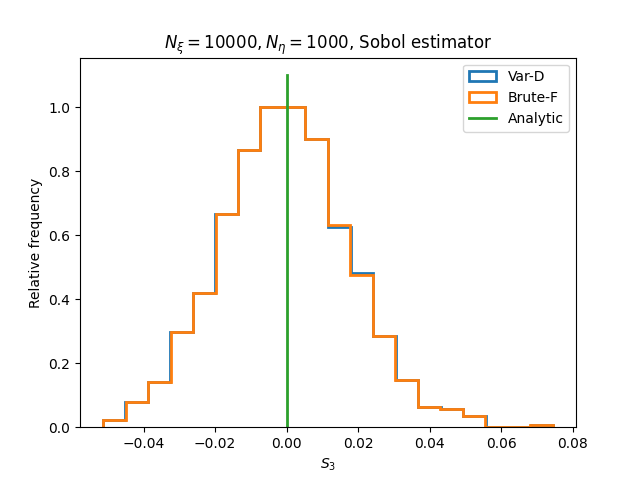
\includegraphics[width=\textwidth]{figures/s3_exp.png}
%         \caption{Computing $\S{3}$ using the Saltelli estimator.}
%         \label{fig:s1}
%     \end{subfigure} \hfill
%     \begin{subfigure}[b]{0.3\textwidth}
%         \centering
%         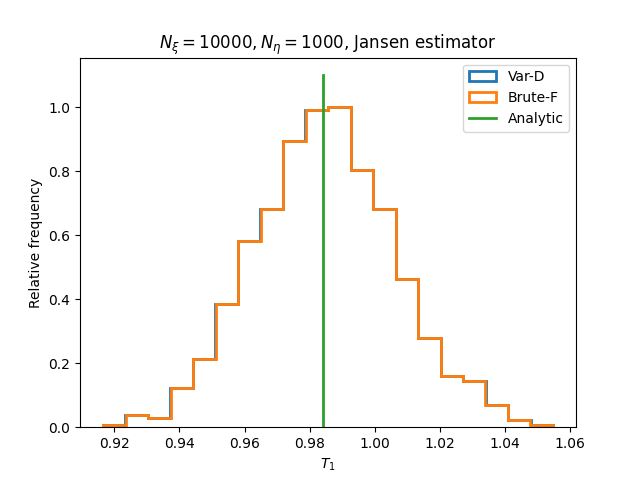
\includegraphics[width=\textwidth]{figures/t1_exp.png}
%         \caption{Computing $\T{1}$ using the Saltelli estimator.}
%         \label{fig:s1}
%     \end{subfigure} \hfill
%     \begin{subfigure}[b]{0.3\textwidth}
%         \centering
%         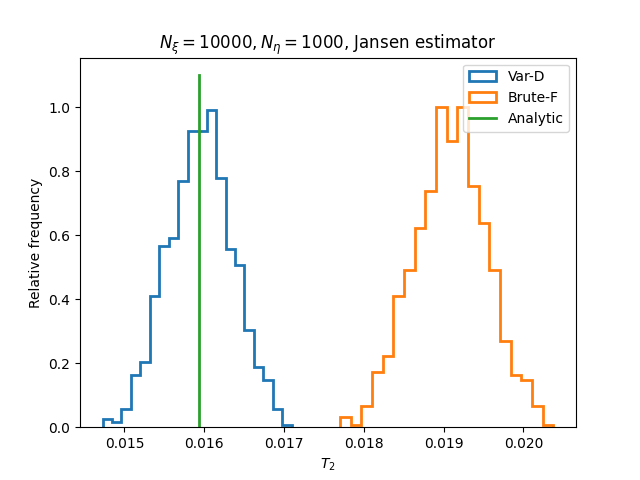
\includegraphics[width=\textwidth]{figures/t2_exp.png}
%         \caption{Computing $\T{2}$ using the Saltelli estimator.}
%         \label{fig:s1}
%     \end{subfigure} \hfill
%     \begin{subfigure}[b]{0.3\textwidth}
%         \centering
%         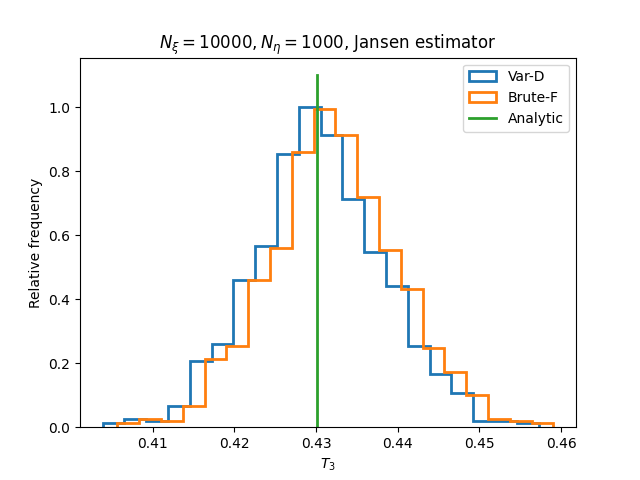
\includegraphics[width=\textwidth]{figures/t3_exp.png}
%         \caption{Computing $\T{3}$ using the Saltelli estimator.}
%         \label{fig:s1}
%     \end{subfigure} \hfill
%     \caption{Comparing the distributions of first- and total-order indices with $\Neta$ increased $200x$ vs Fig.~\ref{fig:ishigami_low}. PDF created with 1\,000 repetitions. Analytic indices reported as solid vertical line.}
% 	\label{fig:ishigami_high}
% \end{figure}

\subsection{Radiation transport test problem}
We next perform GSA on a test neutron transport problem solved using Monte Carlo radiation transport methods~\cite{lux-koblinger-90}. 
The problem is based on the steady-state C5G7 benchmark, a nuclear reactor benchmark developed by the OECD/NEA~\cite{c5g7-2005}. 
We simplify the design by reducing to one dimension in space with three materials: uranium dioxide (UO$_2$) fuel, water moderator, and a control rod. 
There is a constant source, uniform in energy across all groups, at the spatial halfway point.
The neutron energy spectrum is divided into 7 energy groups and we use the cross-sections from the C5G7 benchmark.
Parameter uncertainty is introduced in five independent factors: the densities of 1) the fuel, 2) the moderator, and 3) the control rod were allowed to vary uniformly $\pm 70\%$; 4) the ratio of fuel-width to moderator-width and 5) the control-rod thickness were both allowed to vary uniformly between 0.2 and 0.8. 
We define two quantities of interest as a function of space: the scalar flux of the first two energy groups, $\phi_F (x)$, and the scalar flux of the remaining five energy groups $\phi_S(x)$.

For reference, using $\Nxi=5 \times 10^5$ and $\Neta=10^5$, Figure~\ref{fig:flux} shows $\phi_F (x)$ and $\phi_S (x)$. Figure~\ref{fig:indices} shows the full set of first- and total- order indices for both QoIs.
At such a high $\Neta$, the lines for $\pollSsalt{i}$ and $\pollTsalt{i}$ overlap exactly with those of $\unpollSsalt{i}$ and $\unpollTsalt{i}$, respectively.
The faster group flux $\phi_F$ is most sensitive across space to $\xi_2$, the density of the moderator, which is understandable as the density of the moderator will greatly impact the number of neutrons and their energies everywhere in the problem. 
The control rod's density ($\xi_3$) and thickness ($\xi_5$) are most impactful for the slower group flux, with both having large inflection points at the nominal moderator--control rod boundary at $x=1.5$.
This is understandable as the control rod is a primarily thermal absorber.

\begin{figure}[ht]
    \centering
    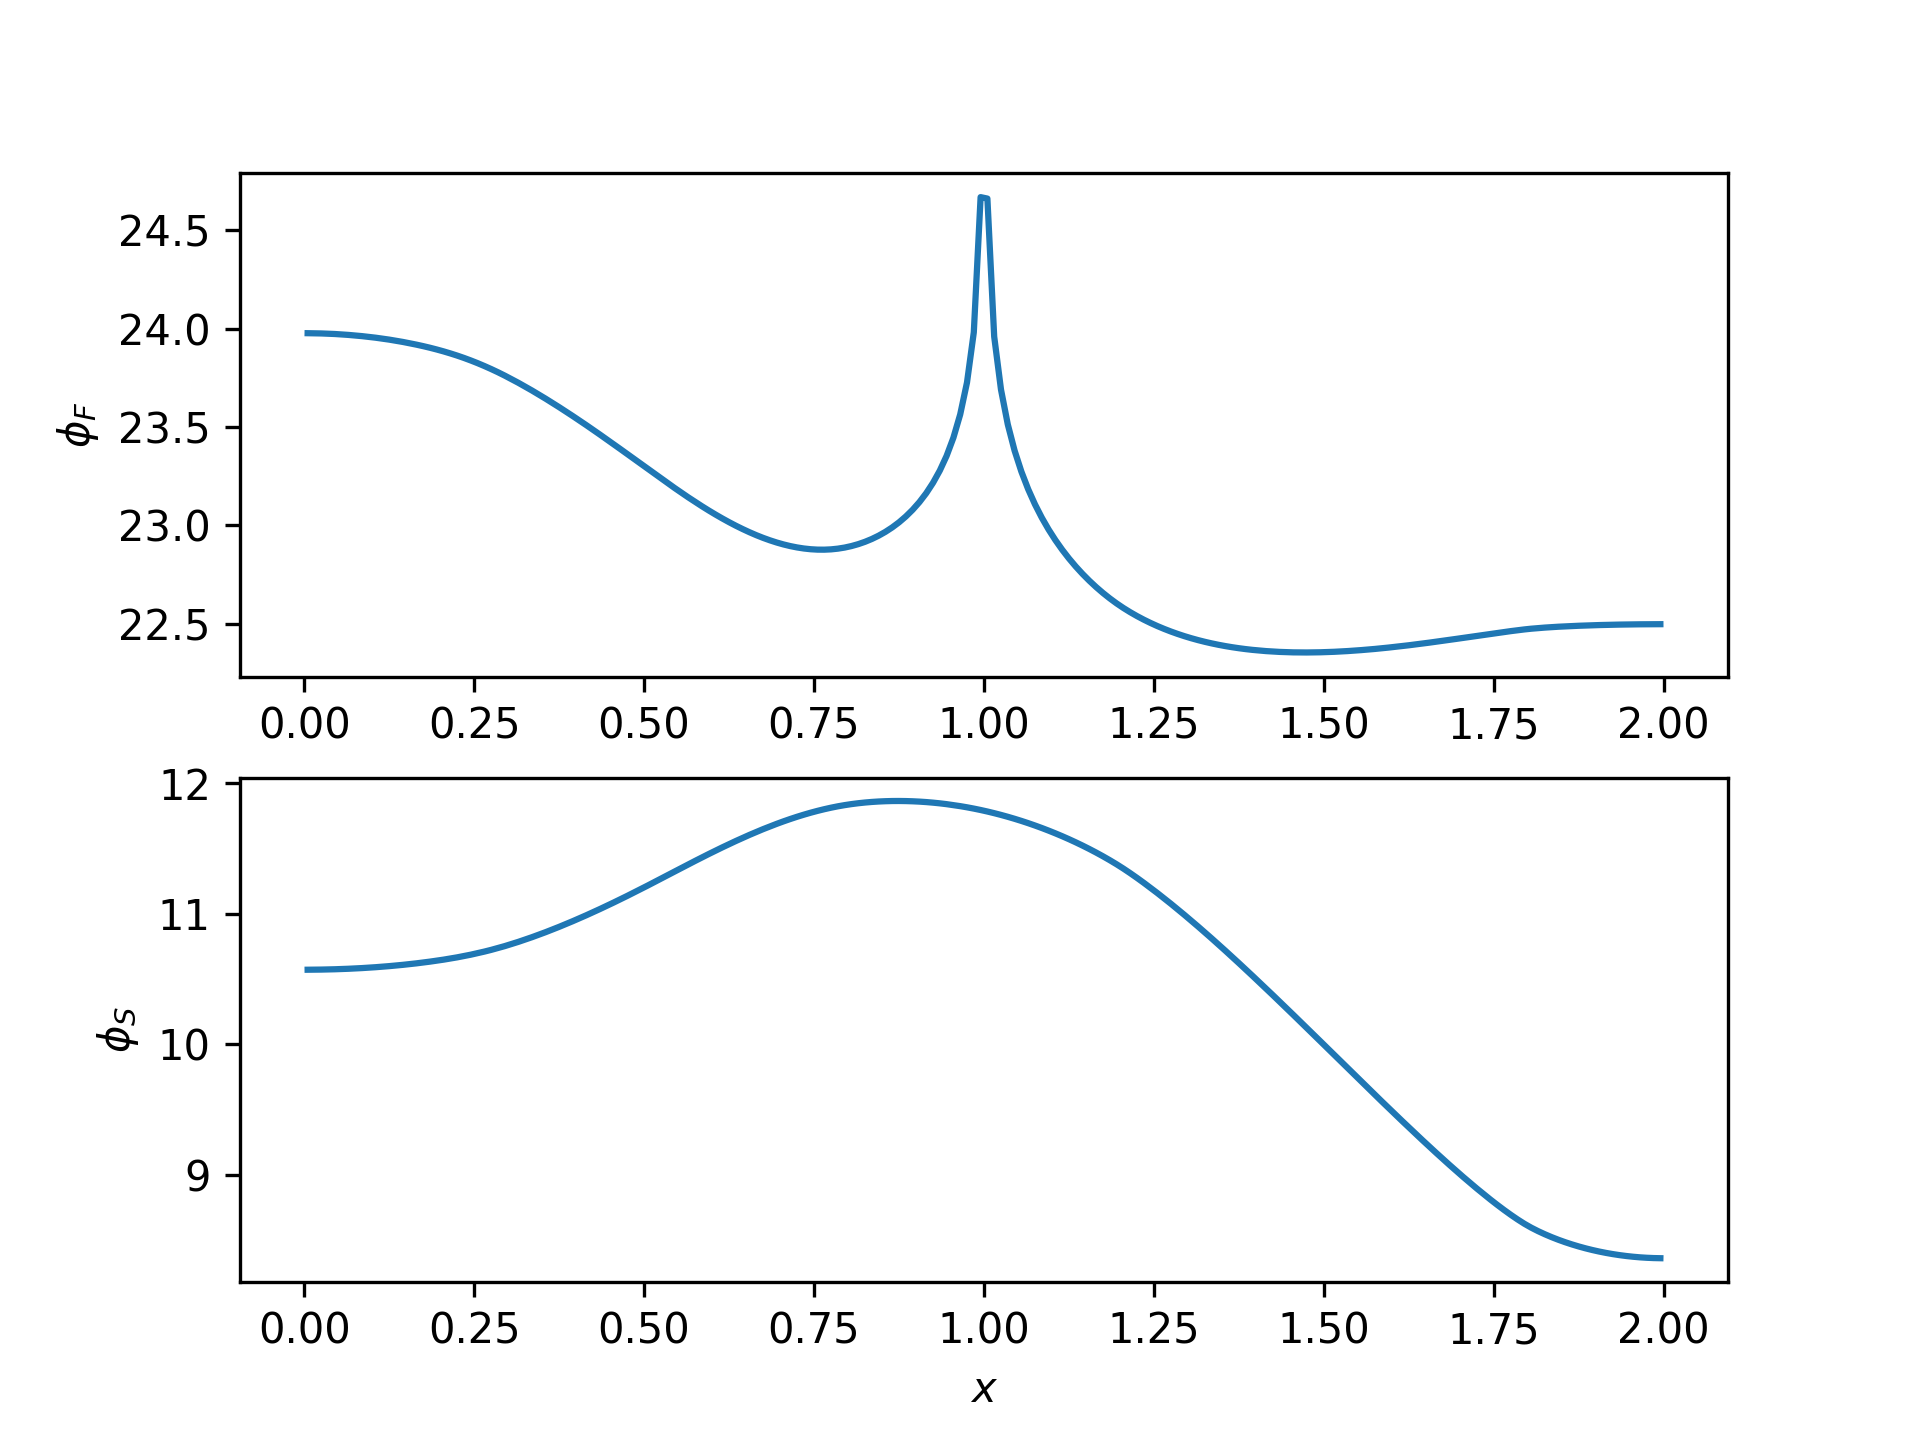
\includegraphics{figures/flux.png} 
    \caption{Average scalar flux with five uncertain parameters using $\Nxi=5 \times 10^5$, $\Neta=10^5$.}
    \label{fig:flux}
\end{figure}

\begin{figure}[ht]
    \centering
    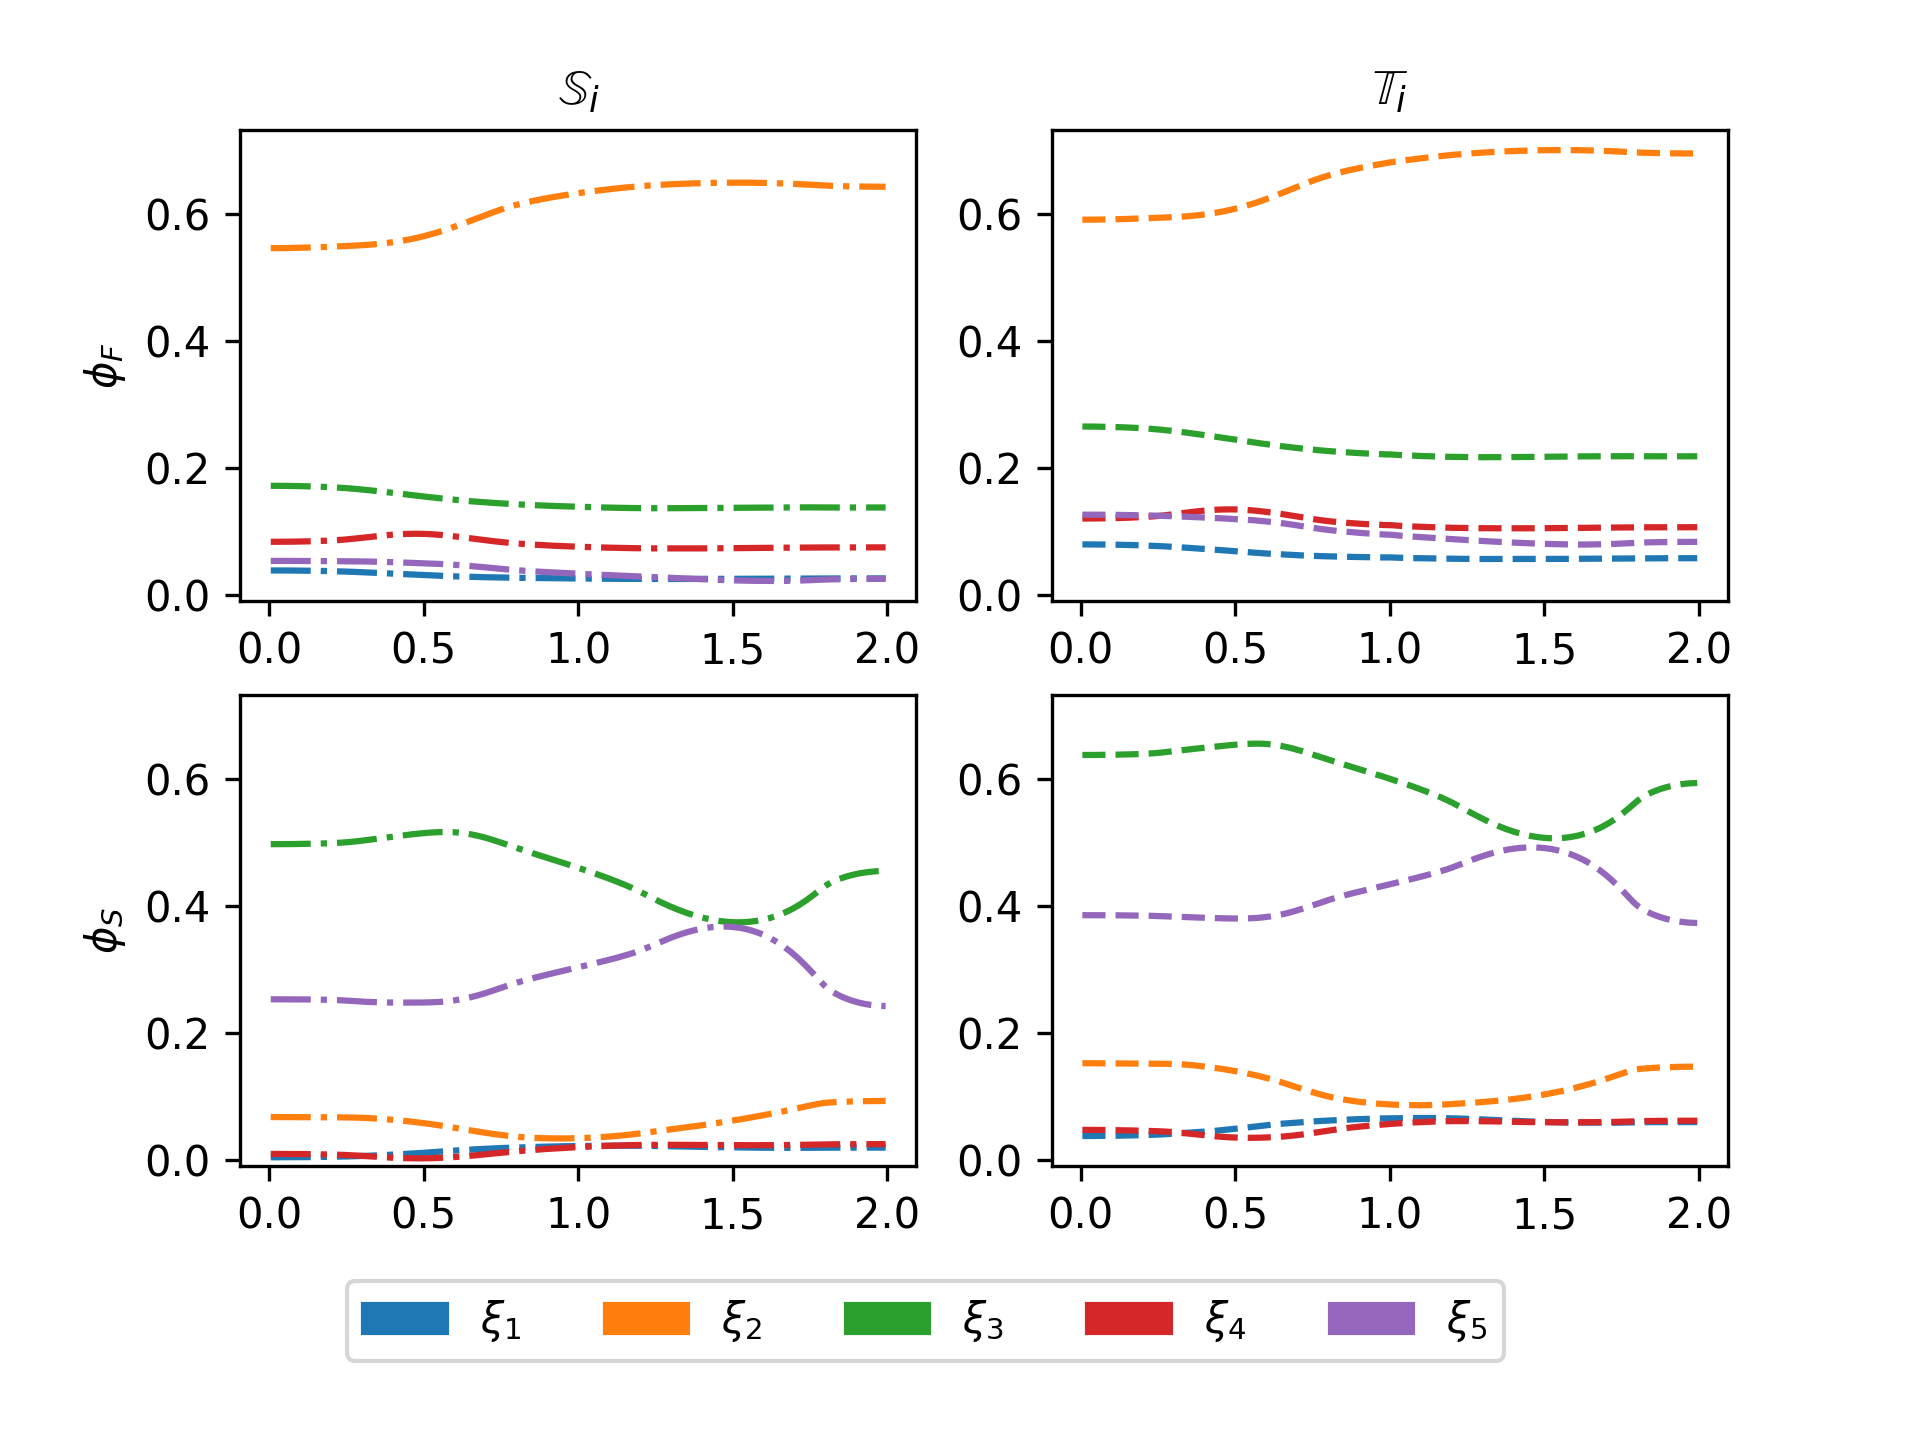
\includegraphics{figures/indices.png}
    \caption{Full set of first- and total- order indices of $\phi_F$ and $\phi_S$ using $\Nxi=5 \times 10^5$, $\Neta=10^5$. Standard and corrected estimators exactly overlap. Uncertain factors: the densities of 1) the fuel, 2) the moderator, 3) and the control rod were allowed to vary uniformly $\pm 70\%$; 4) the ratio of fuel-width to moderator-width and 5) the control-rod thickness were both allowed to vary uniformly between 0.2 and 0.8. }
    \label{fig:indices}
\end{figure}

To see the effect of the variance deconvolution correction, we compare the MSE of the standard and corrected estimators.
In Figure~\ref{fig:mse-fo-fast}, we consider a constant computational cost $\C = \left( \Nxi \times \Neta \right) = 5 \times 10^5$ in two different combinations of $\Nxi$ and $\Neta$.
In the first combination, $\left( \Nxi, \Neta \right) = \left( 5 \times 10^3, 10^2 \right)$, we see that the MSE of the standard estimator is clearly lower than that of the var-d estimator for $\S{1}$ and $\S{5}$. 
Both of these indices are very close to zero (see Figure~\ref{fig:indices}); in this case, the higher variance of the var-d estimator outweighs the bias of the standard estimator.
In the second combination, we have increased $\Nxi$ by a factor of 10 and decreased $\Neta$ by the same factor to keep $\C$ constant.
The variance deconvolution estimator benefits from this configuration, with an MSE that is lower than that of the standard estimator at most locations in $x$. 

This pattern is consistent across QoIs: when indices are close to zero the variance of the variance deconvolution estimator can outweigh the bias of the standard estimator, and for a constant $\C$ the variance deconvolution estimator generally benefits from increasing the $\Nxi$ at the expense of decreasing $\Neta$. 
In Figure~\ref{fig:mse-fo-slow}, we see this for $\S{i} \left[ \phi_S \right]$.
For estimating $\T{i}$, the correction in both the numerator and denominator makes the difference between the standard and variance deconvolution estimators more drastic.
In Figures~\ref{fig:mse-to-fast} and~\ref{fig:mse-to-slow}, we see that the variance deconvolution estimator outperforms the standard across $x$ for both $\phi_F$ and $\phi_S$.

\begin{figure}
    \centering
    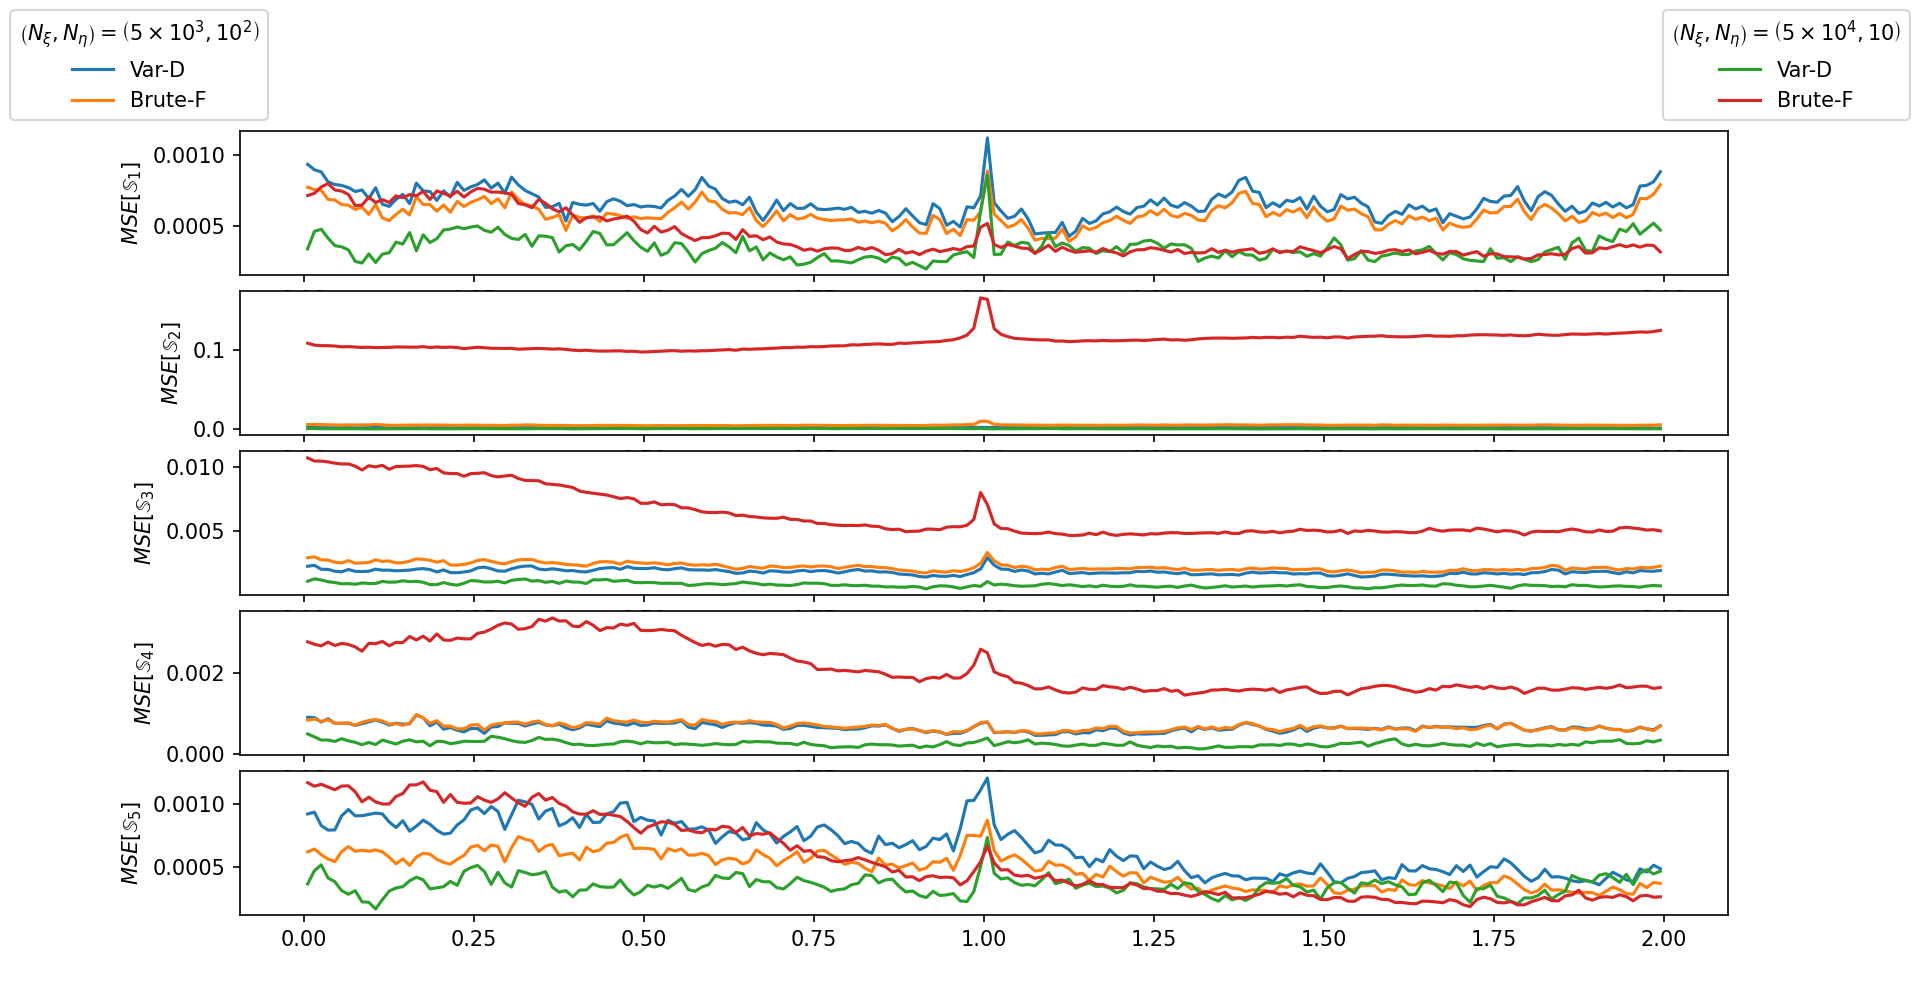
\includegraphics[width=\textwidth]{figures/mse_firstorder_fast.png}
    \caption{$MSE\left[\S{i}\right]$ for $\phi_F$, constant computational cost $\C = \left( \Nxi \times \Neta \right) = 5 \times 10^5$.}
    \label{fig:mse-fo-fast}
\end{figure}

\begin{figure}
    \centering
    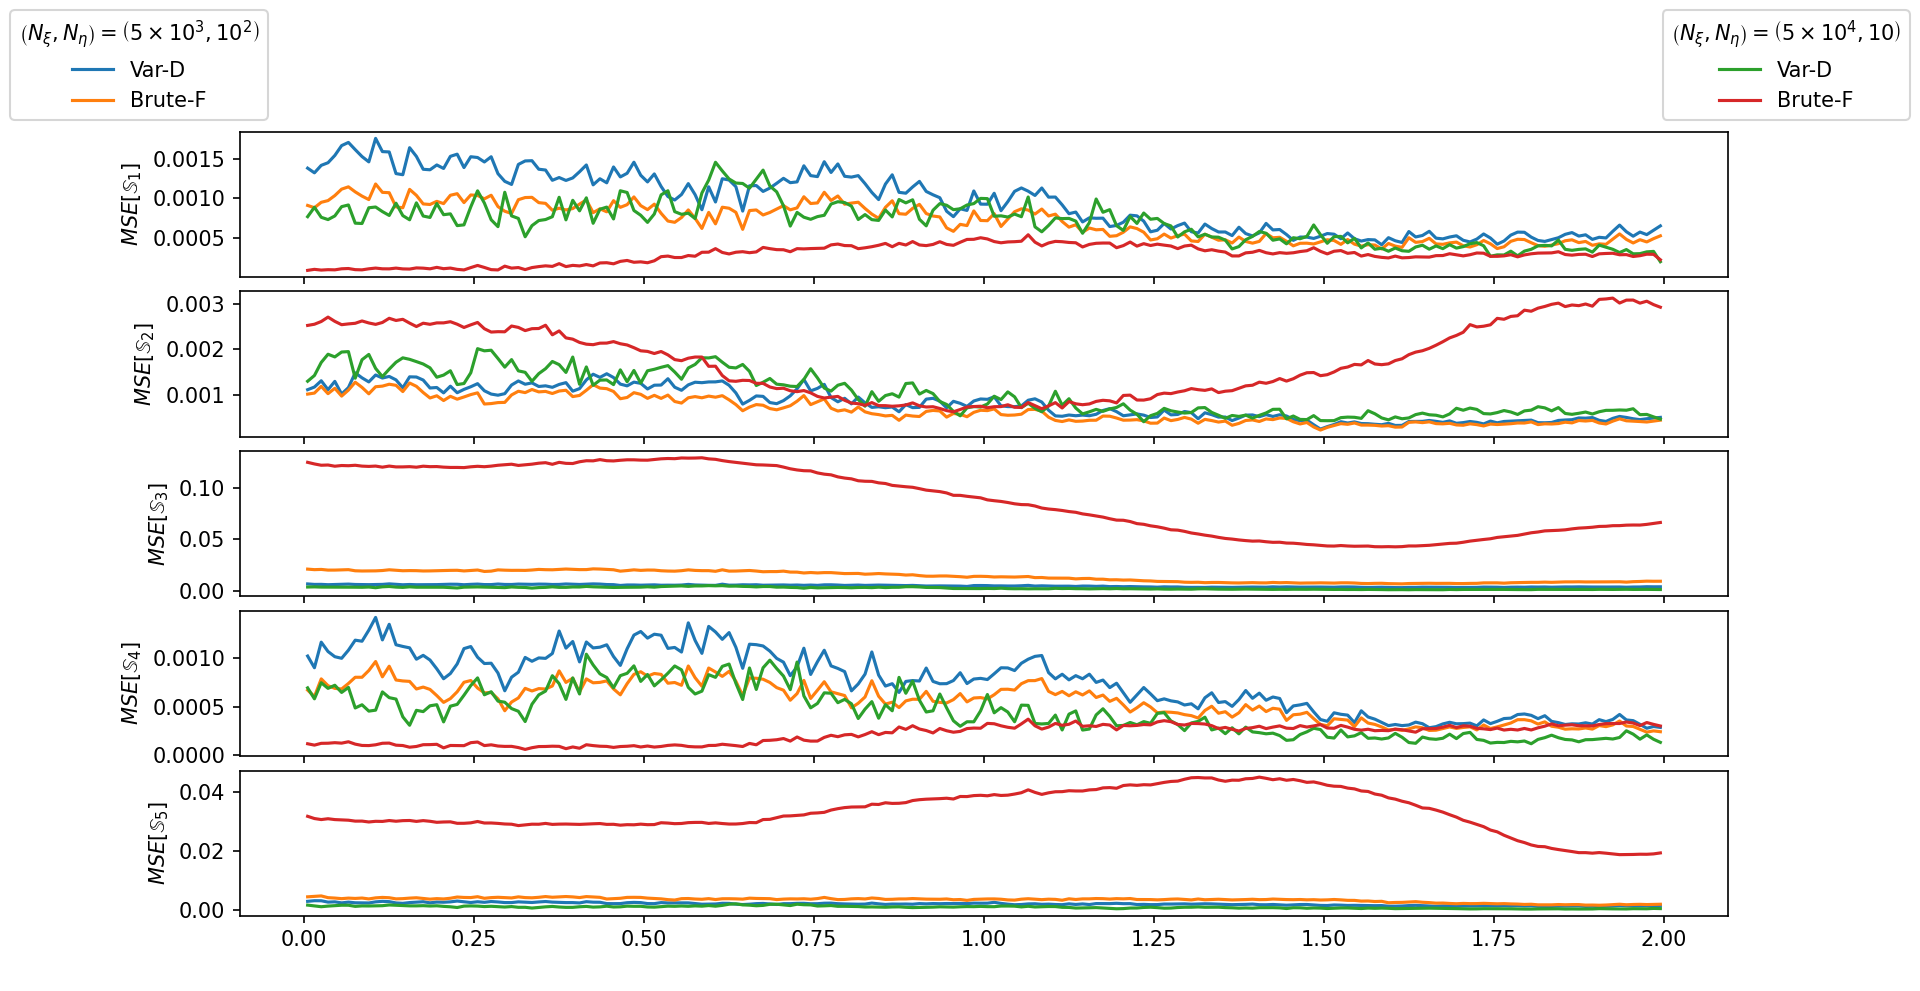
\includegraphics[width=\textwidth]{figures/mse_firstorder_slow.png}
    \caption{$MSE\left[\S{i}\right]$ for $\phi_S$, constant computational cost $\C = \left( \Nxi \times \Neta \right) = 5 \times 10^5$.}
    \label{fig:mse-fo-slow}
\end{figure}

\begin{figure}
    \centering
    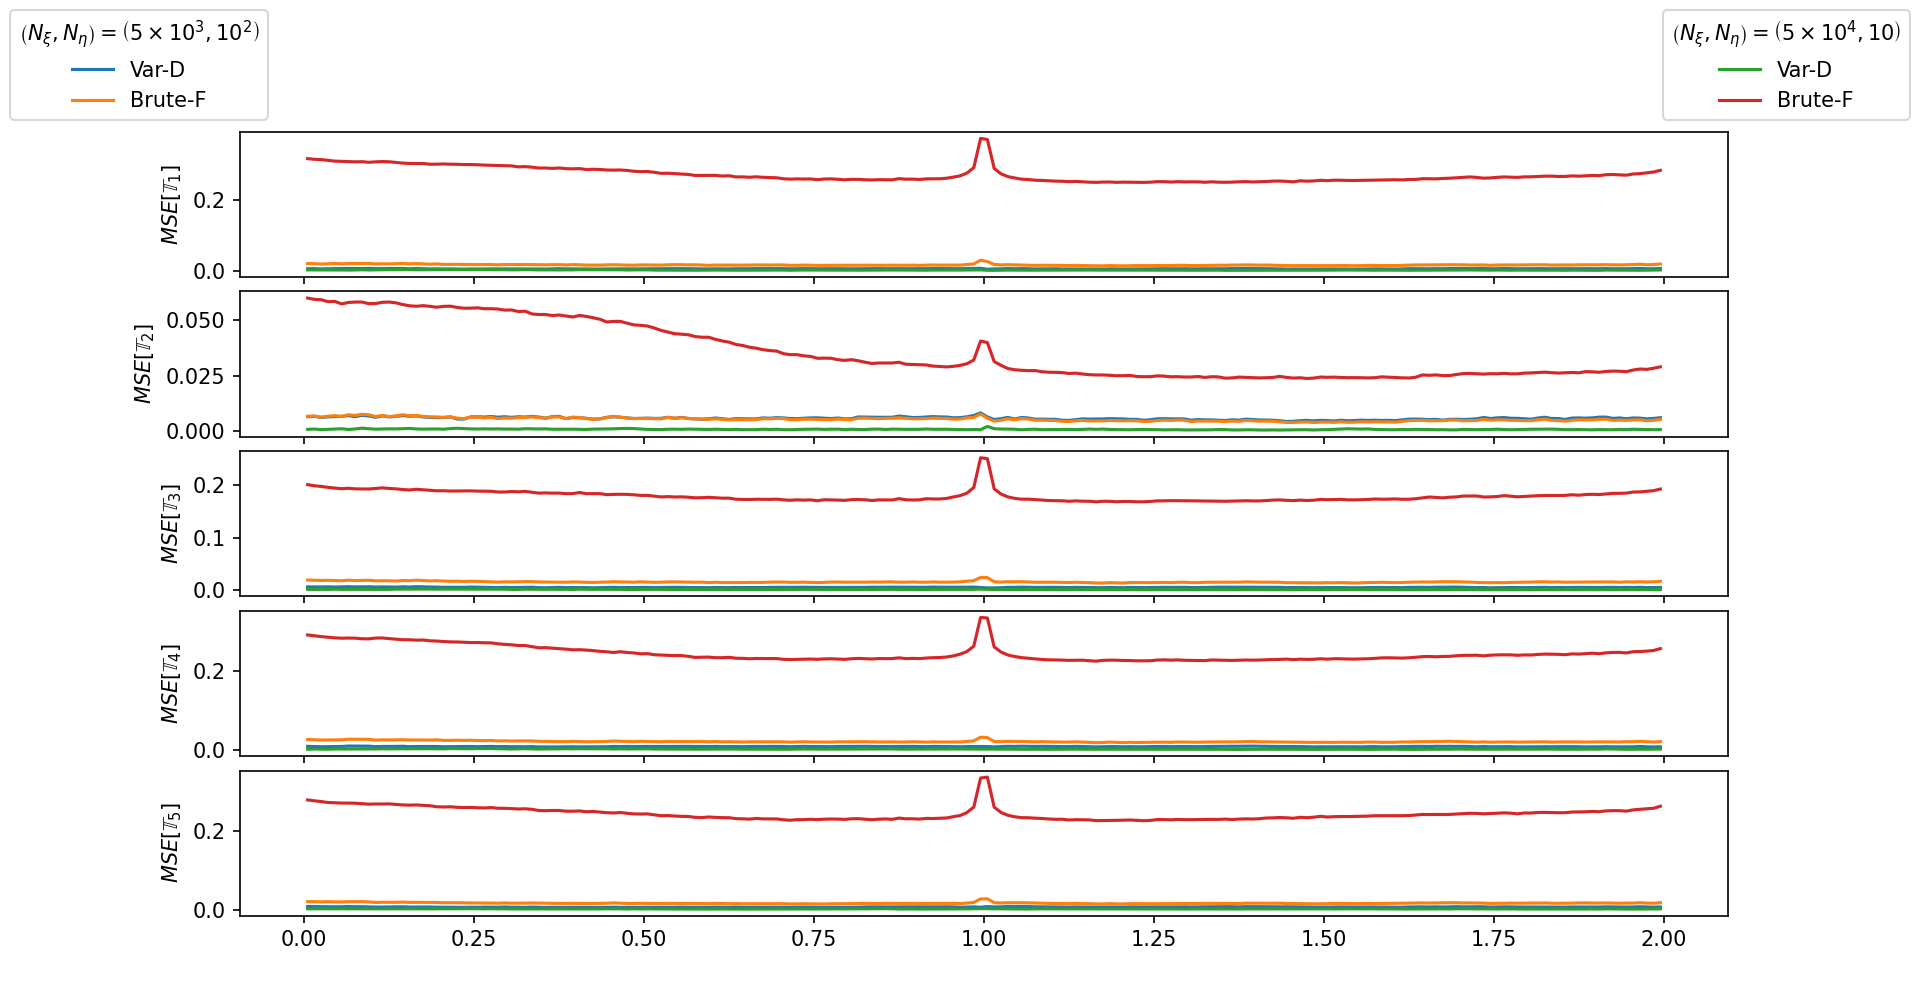
\includegraphics[width=\textwidth]{figures/mse_totalorder_fast.png}
    \caption{$MSE\left[\T{i}\right]$ for $\phi_F$, constant computational cost $\C = \left( \Nxi \times \Neta \right) = 5 \times 10^5$.}
    \label{fig:mse-to-fast}
\end{figure}

\begin{figure}
    \centering
    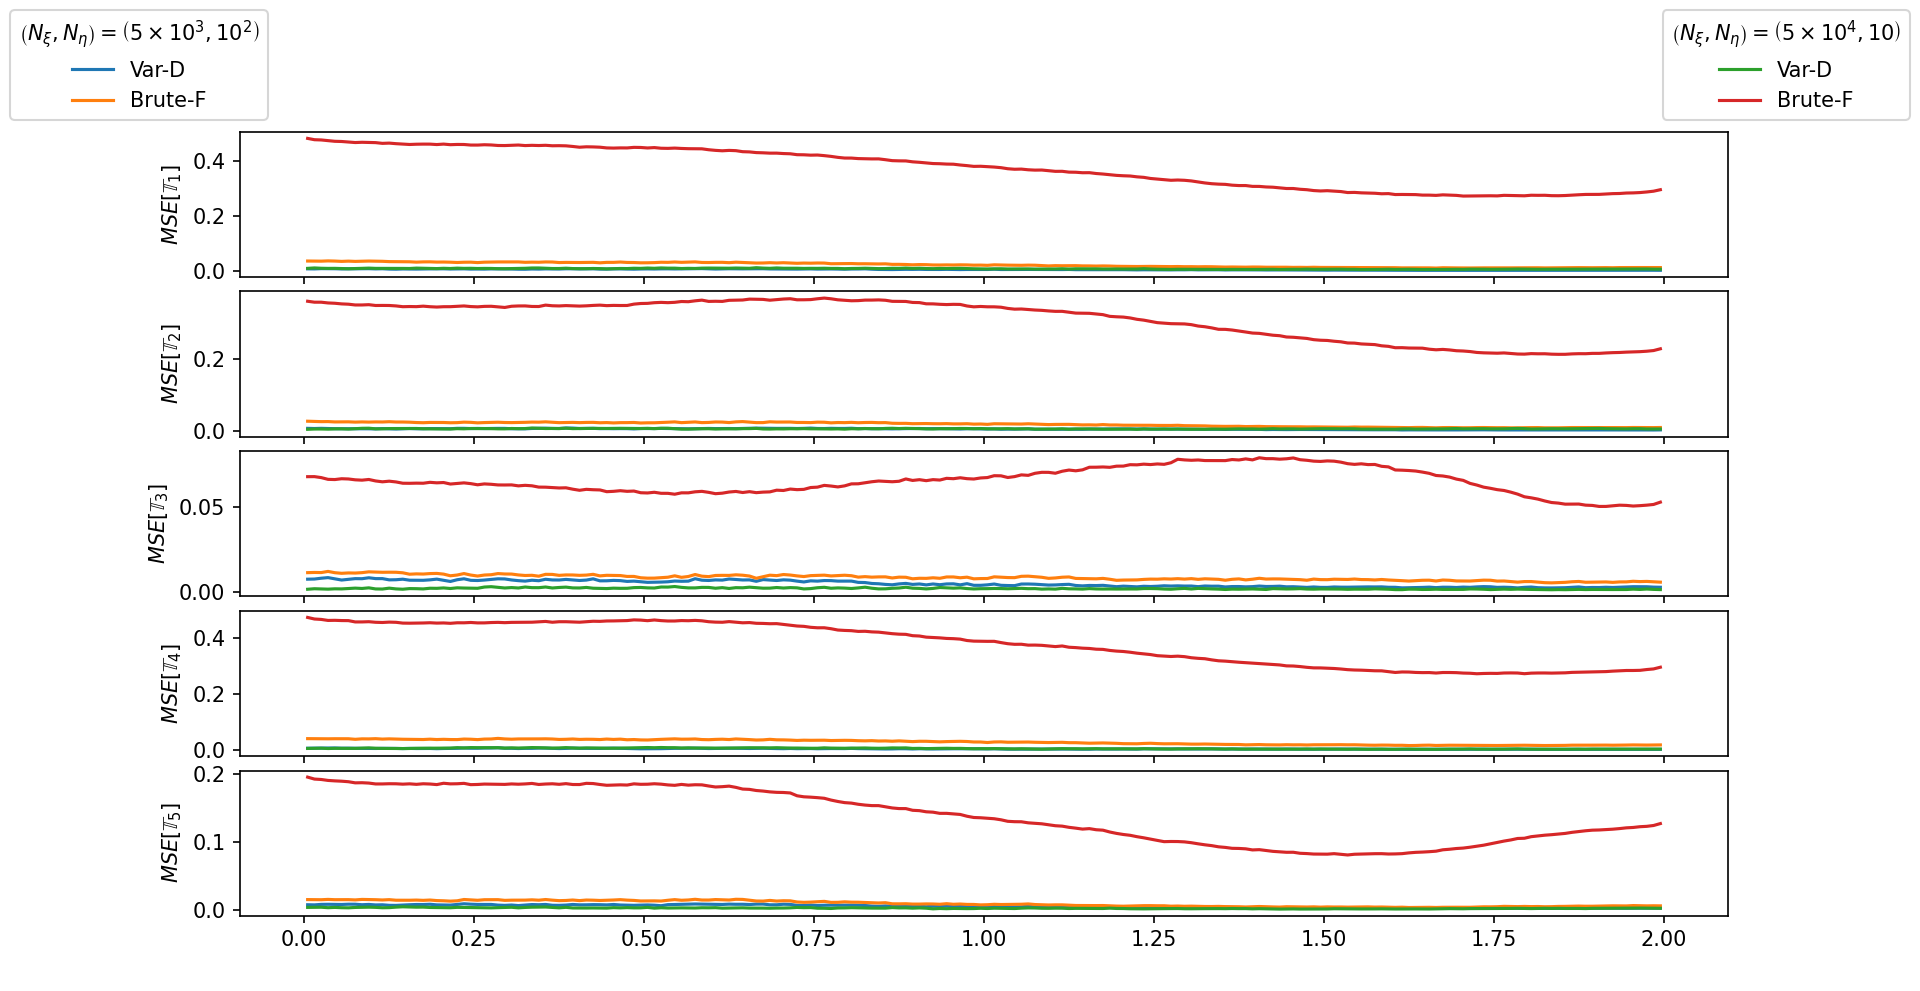
\includegraphics[width=\textwidth]{figures/mse_totalorder_slow.png}
    \caption{$MSE\left[\T{i}\right]$ for $\phi_S$, constant computational cost $\C = \left( \Nxi \times \Neta \right) = 5 \times 10^5$.}
    \label{fig:mse-to-slow}
\end{figure}

We have shown, in this example and the analytic test case, that when increasing computational cost for more accurate estimates of $\S{i}$ and $\T{i}$, putting those computational resources towards increasing $\Nxi$ with the variance deconvolution estimator will improve the accuracy of indices that are not near zero.